\documentclass[11pt]{article}

\usepackage{acl}
\usepackage{times}
\usepackage{latexsym}
\usepackage[T1]{fontenc}
\usepackage[utf8]{inputenc}
\usepackage{microtype}
\usepackage{inconsolata}
\usepackage{graphicx}
\usepackage{booktabs}
\usepackage{amsmath}
\usepackage{array}
\usepackage{xcolor}
\usepackage{tikz}
\usetikzlibrary{arrows.meta,positioning}

\newcommand{\task}{\textsc{AstroCLIMB}}
\newcommand{\sfclass}{\texttt{same\_figure}}
\newcommand{\spclass}{\texttt{same\_paper}}
\newcommand{\rpclass}{\texttt{related\_papers}}
\newcommand{\upclass}{\texttt{unrelated\_papers}}

\title{Syed Mohaiminul Hoque at AstroCLIMB 2026:\\
Parameter-Efficient Adaptation of Qwen3-VL for Astronomy Citation Linking}

\author{Syed Mohaiminul Hoque \\
  Center for Computational and Data Sciences \\
  Independent University, Bangladesh \\
  \texttt{syedmuhaimintahsin@gmail.com}}

\begin{document}
\maketitle

\begin{abstract}
We describe the solo submission of team \emph{Syed Mohaiminul Hoque} to the \task{} shared task at WASP 2026.  The task requires classifying a pair of astronomy figures and/or captions as the same figure, from the same paper, from citation-related papers, or from unrelated papers.  Our system casts classification as constrained next-token prediction with Qwen3-VL and adapts the model using 4-bit quantization and low-rank adapters.  On the 10,000-pair Kaggle test set, three Qwen3-VL-8B models with language-attention adapters obtain 0.73230--0.73307 macro-F1 individually.  Averaging their four-class probabilities raises the score to 0.73604, and masking the impossible same-figure class for caption--caption and image--image pairs produces 0.73725 and third place among 11 teams on the final leaderboard.  This paper documents empirical system engineering rather than proposing a new learning algorithm; broader visual adaptation, restricted-loss blending, and citation-focused auxiliary training do not improve the result.
\end{abstract}

\section{Introduction}

Scientific figures condense results that are difficult to recover with text-only indexing.  The \task{} shared task asks systems to partially reconstruct an astronomy citation graph using only figures and captions \citep{astroclimb2026}.  Unlike conventional document classification, the input is a pair of heterogeneous objects: either object may be an image or a caption, and the target is a symmetric relation between their source papers.

Modern vision--language models (VLMs) offer a natural interface for such mixed inputs.  However, full fine-tuning remains expensive, especially on the two NVIDIA T4 GPUs available in a standard Kaggle environment.  We therefore formulate the task as instruction-following with four possible answer tokens and use QLoRA \citep{dettmers2023qlora} to adapt Qwen3-VL \citep{bai2025qwen3vl}.

We develop a uniform multimodal pipeline with random object swapping; compare scale, loss normalization, adapter coverage, and seed variation; and analyze both a balanced validation split and a negative auxiliary-training result.  Our three-seed probability ensemble with a modality constraint reaches 0.73725 test macro-F1, with the \spclass{}--\rpclass{} distinction remaining the main difficulty.  Code, notebooks, and artifacts are available at \url{https://github.com/SyedT1/Astroclimb-sharedtask}.

\section{Related Work}

Scientific-figure research commonly studies caption generation or cross-modal retrieval.  SciCap introduced a large figure--caption corpus and captioning baselines \citep{hsu2021scicap}; SciMMIR benchmarks retrieval over 530K scientific image--text pairs \citep{wu2024scimmir}.  Chart retrieval also shows value in combining visual, textual, and derendered table evidence \citep{nowak2024chartretrieval}.  \task{} instead predicts provenance relations rather than retrieving a matching caption.

SPECTER2 learns citation-informed scientific-document representations \citep{cohan2020specter,singh2023scirepeval}; SigLIP2 and DINOv3 provide cross-modal and self-supervised visual features \citep{tschannen2025siglip2,simeoni2025dinov3}.  We compare their frozen features with our VLM approach.  Casting labels as answer tokens is related to pattern-based classification \citep{schick2021pet}; our contribution is a carefully evaluated shared-task system combining this interface with QLoRA, ensembling, and a task-valid constraint.

\begin{figure*}[t]
\centering
\resizebox{\textwidth}{!}{%
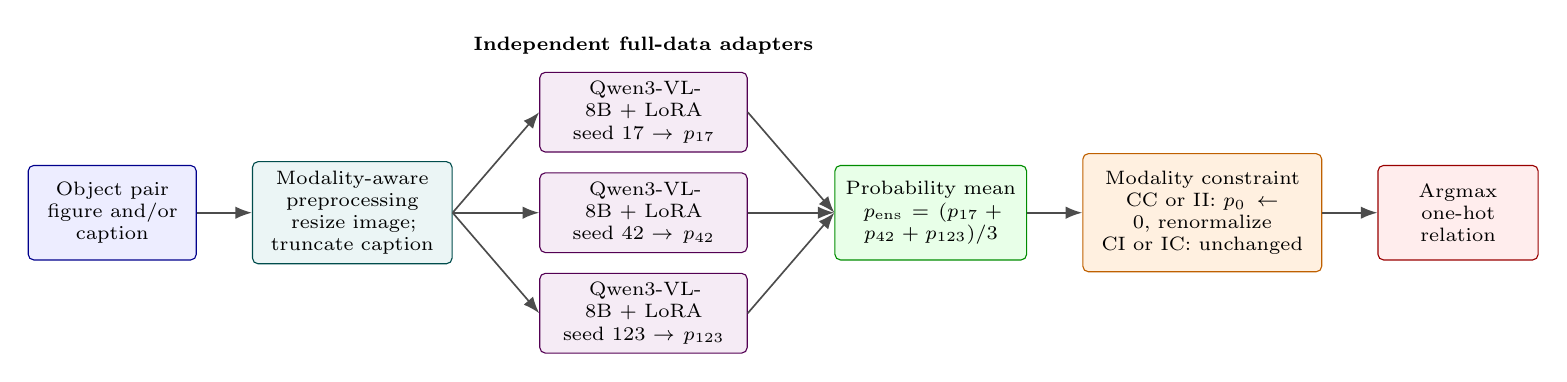
\begin{tikzpicture}[
    node distance=6mm and 7mm,
    flow/.style={-{Latex[length=2.1mm]}, semithick, draw=black!70},
    stage/.style={draw=blue!55!black, rounded corners=2pt, fill=blue!7,
        align=center, minimum height=12mm, text width=19mm, font=\scriptsize},
    prep/.style={draw=teal!60!black, rounded corners=2pt, fill=teal!8,
        align=center, minimum height=12mm, text width=23mm, font=\scriptsize},
    model/.style={draw=violet!65!black, rounded corners=2pt, fill=violet!8,
        align=center, minimum height=9mm, text width=24mm, font=\scriptsize},
    combine/.style={draw=green!55!black, rounded corners=2pt, fill=green!9,
        align=center, minimum height=12mm, text width=22mm, font=\scriptsize},
    constraint/.style={draw=orange!75!black, rounded corners=2pt, fill=orange!12,
        align=center, minimum height=15mm, text width=28mm, font=\scriptsize},
    output/.style={draw=red!60!black, rounded corners=2pt, fill=red!7,
        align=center, minimum height=12mm, text width=18mm, font=\scriptsize}
]
\node[stage] (input) {Object pair\\figure and/or caption};
\node[prep, right=of input] (preprocess) {Modality-aware preprocessing\\resize image; truncate caption};
\node[model, right=11mm of preprocess] (seed42) {Qwen3-VL-8B + LoRA\\seed 42 $\rightarrow p_{42}$};
\node[model, above=2.5mm of seed42] (seed17) {Qwen3-VL-8B + LoRA\\seed 17 $\rightarrow p_{17}$};
\node[model, below=2.5mm of seed42] (seed123) {Qwen3-VL-8B + LoRA\\seed 123 $\rightarrow p_{123}$};
\node[font=\scriptsize\bfseries, above=1mm of seed17] {Independent full-data adapters};
\node[combine, right=11mm of seed42] (mean) {Probability mean\\$p_{\mathrm{ens}}=(p_{17}+p_{42}+p_{123})/3$};
\node[constraint, right=of mean] (mask) {Modality constraint\\CC or II: $p_0\leftarrow0$, renormalize\\CI or IC: unchanged};
\node[output, right=of mask] (output) {Argmax\\one-hot relation};
\draw[flow] (input) -- (preprocess);
\draw[flow] (preprocess.east) -- (seed17.west);
\draw[flow] (preprocess.east) -- (seed42.west);
\draw[flow] (preprocess.east) -- (seed123.west);
\draw[flow] (seed17.east) -- (mean.west);
\draw[flow] (seed42.east) -- (mean.west);
\draw[flow] (seed123.east) -- (mean.west);
\draw[flow] (mean) -- (mask);
\draw[flow] (mask) -- (output);
\end{tikzpicture}
}
\caption{Inference pipeline of the best system.  Three full-vocabulary Qwen3-VL-8B language-attention QLoRA models produce four-class probabilities.  Equal averaging reduces seed variance, after which a deterministic modality mask removes the impossible \sfclass{} option from caption--caption and image--image pairs.}
\label{fig:pipeline}
\end{figure*}

\section{Task and Data}

Each example is a pair $x_i=(o_{i1},o_{i2})$.  An object is either an English figure caption or a base64-encoded scientific figure.  The four mutually exclusive classes are: (0) \sfclass{}, when the objects are the image and caption of one figure; (1) \spclass{}, when they are different objects from one paper; (2) \rpclass{}, when one source paper cites the other; and (3) \upclass{}.  The relation is symmetric under exchanging the two objects.

The Kaggle release contains 10,000 labeled training pairs and 10,000 test pairs.  Training labels are distributed $(1000,3000,3000,3000)$ in class order.  The official metric is macro-averaged F1,
\begin{equation}
F_{1,\mathrm{macro}}=\frac{1}{4}\sum_{c=0}^{3}F_{1,c},
\end{equation}
so performance on the less frequent \sfclass{} class contributes equally.  The broader collection contains 94,233 figure--caption records with citation metadata \citep{astroclimbdataset2026}; we use it only for the auxiliary experiment in Section~\ref{sec:auxiliary}.

For controlled experiments, we reserve 200 examples per class using seed 42, producing a balanced 800-pair validation set and 9,200 training pairs.  Full-data systems use all 10,000 labeled pairs.  We do not use test metadata, external DOI lookup, or hidden labels.

\begin{table*}[t]
\centering
\footnotesize
\setlength{\tabcolsep}{3pt}
\begin{tabular}{llrlr}
\toprule
Backbone & Training setup & Epochs & Adapter coverage & Test macro-F1 \\
\midrule
Frozen encoders & SPECTER2/SigLIP2/DINO + features & --- & modality CatBoost & 0.48279 \\
Qwen3-VL-4B & balanced 5K, $\mathcal{L}_{\mathrm{vocab}}$ & 1.0 & language attention & 0.67856 \\
Qwen3-VL-4B & full 10K, $\mathcal{L}_{\mathrm{vocab}}$ & 1.0 & language attention & 0.70751 \\
Qwen3-VL-4B & 9.2K, $\mathcal{L}_{4}$ & 2.0 & language attention & 0.71453 \\
Qwen3-VL-4B & full 10K, $\mathcal{L}_{\mathrm{vocab}}$ & 1.0 & language + visual projectors & 0.71016 \\
Qwen3-VL-4B & full 10K, $\mathcal{L}_{\mathrm{vocab}}$ & 1.0 & all linear layers & 0.71202 \\
Qwen3-VL-8B & full 10K, $\mathcal{L}_{\mathrm{vocab}}$, seed 42 & 1.0 & language attention & 0.73230 \\
Qwen3-VL-8B & full 10K, $\mathcal{L}_{\mathrm{vocab}}$, seed 123 & 1.0 & language attention & 0.73250 \\
Qwen3-VL-8B & full 10K, $\mathcal{L}_{\mathrm{vocab}}$, seed 17 & 1.0 & language attention & 0.73307 \\
Qwen3-VL-8B & full 10K, $\mathcal{L}_{4}$ & 1.5 & language attention & 0.73032 \\
Qwen3-VL-8B & three-seed probability ensemble & 1.0 & language attention & 0.73604 \\
Qwen3-VL-8B & 75\% ensemble + 25\% restricted & --- & probability blend & 0.73590 \\
Qwen3-VL-8B & ensemble + modality mask & --- & deterministic constraint & \textbf{0.73725} \\
\bottomrule
\end{tabular}
\caption{Final Kaggle leaderboard results.  ``Full 10K'' denotes all labeled pairs; the 9.2K run retains 800 validation pairs.  The final three rows are derived systems.}
\label{tab:main}
\end{table*}

\section{System Description}

\subsection{Input representation}

We use instruction-tuned Qwen3-VL-4B and Qwen3-VL-8B checkpoints.  A system message defines the four relations and assigns them digits 0--3.  The user message then presents Object~1 and Object~2 in their native modalities and asks for one digit.  Captions are limited to 3,000 characters by retaining both their beginning and end.  Images are decoded to RGB and processed within an area range of $256^2$ to $448^2$ pixels.  This cap is important for fitting the 8B model on T4 hardware.

Because the relation is symmetric, each training pair is randomly swapped with probability 0.5 without changing its label.  We do not use swap test-time augmentation in the submitted systems.

\subsection{QLoRA adaptation}

We load the backbone in 4-bit NormalFloat (NF4) format with double quantization and FP16 computation.  Low-rank adaptation \citep{hu2022lora} modifies a frozen weight $W_0$ as
\begin{equation}
W_{\mathrm{eff}}=Q_{\mathrm{NF4}}(W_0)+\frac{\alpha}{r}BA,
\end{equation}
where $r=16$, $\alpha=32$, and LoRA dropout is 0.05.  Our main systems adapt language-attention \texttt{q/k/v/o} projections; we also test adding visual-merger projectors or adapting all eligible linear layers.

Training uses two-process distributed data parallelism, one process per T4.  The per-device batch size is one with eight gradient-accumulation steps, giving a global batch size of 16.  The primary full-data systems train for one epoch with learning rate $10^{-4}$.  The 8B restricted-loss refit uses $5\times10^{-5}$ for 1.5 epochs, selected on the fixed validation split.

\subsection{Classification objectives}

Let $t_c$ be the tokenizer ID for digit $c$, and let $z_{i,v}$ be the logit immediately before the answer.  The full-vocabulary objective supervises only that position:
\begin{equation}
\mathcal{L}_{\mathrm{vocab}}=-\frac{1}{N}\sum_{i=1}^{N}
\log\frac{\exp z_{i,t_{y_i}}}{\sum_{v\in\mathcal{V}}\exp z_{i,v}}.
\end{equation}
We also test $\mathcal{L}_4$, replacing the denominator by the four valid digit tokens.  Inference always selects the largest of those four logits, avoiding unconstrained generation.  Appendix~\ref{sec:objective-details} gives the full restricted-loss, inference, and swap definitions.

\subsection{Probability ensemble and modality constraint}

Figure~\ref{fig:pipeline} summarizes the best system.  We independently train the full-vocabulary 8B configuration with seeds 17, 42, and 123.  If $p_s(c\mid x)$ is the normalized four-class distribution from seed $s$, their equal-weight ensemble is
\begin{equation}
p_{\mathrm{ens}}(c\mid x)=\frac{1}{3}
\sum_{s\in\{17,42,123\}}p_s(c\mid x).
\end{equation}
This is probability averaging rather than majority voting over hard predictions.

The \sfclass{} label is valid only for a cross-modal figure--caption pair.  For caption--caption (CC) and image--image (II) pairs, we impose the task constraint after ensembling:
\begin{equation}
\widetilde p_0=0,\qquad
\widetilde p_c=\frac{p_{\mathrm{ens},c}}{\sum_{j=1}^{3}p_{\mathrm{ens},j}}
\quad(c=1,2,3).
\end{equation}
Cross-modal probabilities remain unchanged.  The mask modifies vectors for 6,000 of 10,000 test rows but changes only seven hard predictions.  We do not use swap test-time augmentation, class-bias calibration, or the restricted-loss model in the final system.

\section{Experiments}

\subsection{Zero-shot baselines}

With the same prompt and 4-bit loading, Qwen3-VL-4B is the strongest zero-shot model at 0.47956 macro-F1; Qwen2.5-VL \citep{bai2025qwen25vl} scores 0.46745.  The frozen-encoder baseline in Table~\ref{tab:main} reaches 0.48279; Appendix~\ref{sec:additional-results} details both baselines.

\subsection{Fine-tuned systems}

Table~\ref{tab:main} summarizes the final-leaderboard results.  Full-data 4B training raises macro-F1 from 0.47956 to 0.70751; the analogous 8B seed-42 model reaches 0.73230.  Replications score 0.73250 and 0.73307, motivating probability averaging.

The best 8B model exceeds the comparable 4B model by 0.02556.  Across three seeds, the mean is $0.73262\pm0.00040$ sample standard deviation (range 0.00077).  Broader 4B adapter coverage adds only 0.00265--0.00451; a visual-projector-only run scores 0.48182 because caption--caption pairs bypass its trainable path.

The restricted-loss comparison also changes the split and epochs.  Its selected 8B checkpoint obtains 0.729164 validation macro-F1; a full-data refit scores 0.73032.  Blending 25\% of its probabilities into the ensemble scores 0.73590, 0.00014 below the raw ensemble.

Probability averaging improves the best seed by 0.00297; the mask adds 0.00121, reaching 0.73725 and third of 11 teams.  Seven predictions move from the impossible \sfclass{} label to \spclass{}, with no extra inference.

\subsection{Controlled validation analysis}

On the balanced 800-pair split, the selected restricted-loss checkpoint obtains 0.72916 macro-F1.  \sfclass{} is easiest and \rpclass{} weakest.  Adding language MLP targets reaches 0.729019 while requiring more resources, supporting attention-only adaptation.  Appendix~\ref{sec:additional-results} gives the per-class results.

\subsection{Citation-focused auxiliary training}
\label{sec:auxiliary}

We construct 20,000 auxiliary examples from the public AstroCLIMB collection \citep{astroclimbdataset2026}, distributed as $(2000,6000,8000,4000)$ in class order.  Class 0 replays training examples with replacement; classes 1--3 pair captions from one DOI, directly citation-linked DOIs, or non-adjacent papers sharing a meaningful title token, with metadata used only for selection.  UUID-pair keys enforce pair-level uniqueness for classes 1--3, and exact normalized-caption matches exclude recoverable validation and test DOIs, although image-only papers cannot be mapped.  This auxiliary stage lowers macro-F1 from 0.72916 to 0.71405, likely because metadata relations need not be visible in the sampled captions; Appendix~\ref{sec:additional-results} gives detailed results.

\section{Error Analysis}

Three patterns emerge.  First, exact figure--caption matching is comparatively tractable because shared entities, values, labels, and panel structure provide direct alignment.  The raw ensemble nevertheless predicts \sfclass{} for seven same-modality pairs, which the mask corrects.  Second, same-paper and citation-related pairs often share topics, making similarity an unreliable proxy for provenance.  Third, image-heavy inputs are harder than text-heavy inputs; modality-level diagnostics are reported in Appendix~\ref{sec:additional-results}.

The result that language-side adaptation outperforms broad visual adaptation is not evidence that figures are unimportant.  Instead, 10,000 labels may be insufficient to tune many visual parameters, while the pretrained visual encoder already supplies useful features.  Better figure-specific pretraining, OCR, and evidence-aware sampling are promising directions.

\section{Efficiency and Reproducibility}

The restricted 8B run trains 15,335,424 parameters for 938 steps in 320.45 minutes, peaking at 11.53~GiB on rank~0.  Two-T4 inference over 10,000 pairs takes 78.15 minutes.  The final system requires three independently trained and inferred adapters, but ensembling and masking are CPU-only.  We use Transformers 4.57.1, PEFT 0.17.1, Accelerate 1.10.1, and bitsandbytes 0.47.0.  The split seed is 42; full-data seeds are 17, 42, and 123.  Appendix~C reports the optimizer, scheduler, checkpoint policy, and output validation.

\section{Conclusion}

Our language-attention QLoRA system constrains Qwen3-VL prediction to four tokens.  One 8B model reaches 0.73307 test macro-F1, three-seed averaging reaches 0.73604, and the modality mask yields 0.73725, ranking third of 11 teams.  Broader visual adaptation, restricted-loss blending, and citation-graph supervision do not improve the result.  Future work should prioritize evidence-visible auxiliary examples and stronger cross-figure textual grounding.

\section*{Limitations}

Most full-data configurations lack local validation, and differences are measured by single final-leaderboard scores.  Final labels and example-level predictions are unavailable, so bootstrap confidence intervals and paired significance tests cannot be computed; the reported seed standard deviation measures run variability, not a confidence interval.  The controlled split uses one seed and may share source papers across partitions because paper identifiers are unavailable.  Some comparisons vary multiple factors, including data size and epoch count.  Caption truncation and image resizing can remove evidence.  Finally, metadata-defined citation relations may be invisible in the presented objects, imposing a task-level ceiling that we do not estimate.

\section*{Ethics Statement}

The system processes public scientific figures and captions supplied for the shared task.  It is a benchmark model, not an authoritative bibliographic database: predicted links can be wrong and should not assign credit, evaluate researchers, or alter citation records without verification.  We use only released data and public task metadata and infer no sensitive personal attributes.  GPU computation is the main environmental cost; 4-bit quantization, LoRA, and constrained one-step inference reduce it relative to full-model training and free-form generation.

\section*{Acknowledgments}

The author thanks the WASP 2026 organizers, NASA ADS, and AstroExplorer for the \task{} benchmark.

\clearpage
\bibliography{references}

\clearpage
\appendix

\section{Objective and Prompt Details}
\label{sec:objective-details}

Because the ground-truth relation is symmetric, each training pair is swapped with probability 0.5:
\begin{equation}
\begin{aligned}
(\tilde{o}_{i1},\tilde{o}_{i2})
&=\begin{cases}
(o_{i2},o_{i1}) & b_i=1,\\
(o_{i1},o_{i2}) & b_i=0,
\end{cases}\\[-2pt]
b_i&\sim\mathrm{Bernoulli}(0.5).
\end{aligned}
\end{equation}
The label is unchanged.  For the restricted objective, the denominator contains only the four valid digit tokens:
\begin{equation}
\mathcal{L}_{4}=-\frac{1}{N}\sum_{i=1}^{N}
\log\frac{\exp z_{i,t_{y_i}}}{\sum_{c=0}^{3}\exp z_{i,t_c}}.
\end{equation}
Regardless of the training objective, inference reads only those digit logits:
\begin{equation}
\hat{y}_i=\arg\max_{c\in\{0,1,2,3\}}z_{i,t_c}.
\end{equation}

The system instruction used in the main runs is:
\begin{quote}\small
You classify the relationship between two objects from astronomy papers.\\
0: The objects are the figure and caption of the same scientific figure.\\
1: The objects are from different figures in the same paper.\\
2: The objects are from different papers and one paper cites the other.\\
3: The objects are from unrelated papers.\\
The relationship is symmetric. Output only one digit: 0, 1, 2, or 3.
\end{quote}
Each object is introduced as either a ``scientific figure'' or a ``figure caption.''  The final user instruction is: ``Classify their relationship. Reply with one digit only.''

\section{Additional Experimental Results}
\label{sec:additional-results}

Our non-generative baseline combines frozen SPECTER2 caption embeddings \citep{singh2023scirepeval}, SigLIP2 image--text embeddings \citep{tschannen2025siglip2}, and DINO visual embeddings \citep{simeoni2025dinov3} with word/character TF--IDF, OCR overlap, and perceptual-hash similarities.  Three modality-specific CatBoost classifiers handle caption--caption, mixed, and image--image pairs.  It is therefore a frozen-feature classifier pipeline, not a SPECTER-only model.  Its submission scores 0.48279 final-leaderboard macro-F1.

\begin{table}[h]
\centering
\small
\begin{tabular}{lr}
\toprule
Model & Test macro-F1 \\
\midrule
Qwen3-VL-4B-Instruct & \textbf{0.47956} \\
Qwen2.5-VL-7B-Instruct & 0.46745 \\
Qwen3-VL-8B-Instruct & 0.40112 \\
\bottomrule
\end{tabular}
\caption{Zero-shot results on the 10,000-pair test set.}
\label{tab:zero}
\end{table}

\begin{table}[h]
\centering
\small
\begin{tabular}{lr}
\toprule
Metric & F1 \\
\midrule
\sfclass{} & 0.92913 \\
\spclass{} & 0.66988 \\
\rpclass{} & 0.53790 \\
\upclass{} & 0.77975 \\
\midrule
Macro average & \textbf{0.72916} \\
\bottomrule
\end{tabular}
\caption{Fixed-split results for restricted-loss 8B QLoRA.}
\label{tab:val}
\end{table}

\begin{table}[h]
\centering
\small
\begin{tabular}{lrr}
\toprule
Metric & Baseline & +Auxiliary \\
\midrule
Macro-F1 & \textbf{0.72916} & 0.71405 \\
\sfclass{} & \textbf{0.92913} & 0.89431 \\
\spclass{} & \textbf{0.66988} & 0.62830 \\
\rpclass{} & 0.53790 & \textbf{0.54067} \\
\upclass{} & 0.77975 & \textbf{0.79293} \\
\bottomrule
\end{tabular}
\caption{Per-class F1 before and after auxiliary training.}
\label{tab:aux}
\end{table}

The auxiliary stage contains 20,000 pairs distributed as $(2000,6000,8000,4000)$, followed by restricted-loss tuning on 9,200 competition pairs.  Its confusion matrix (gold rows, predicted columns) is
\begin{equation}
\begin{bmatrix}
165&30&5&0\\
4&131&62&3\\
0&51&113&36\\
0&5&38&157
\end{bmatrix}.
\end{equation}
The largest confusion is bidirectional between \spclass{} and \rpclass{} (62 and 51 cases).  Auxiliary training improves the two different-paper classes but degrades \sfclass{} and \spclass{}.  Modality-level macro-F1 is 0.72845 on caption--caption, 0.67108 on caption--image, and 0.65102 on image--image pairs.  These values diagnose the auxiliary model, not the full-data submission.

\section{Primary Configuration and Reproducibility}

\begin{table}[h]
\centering
\footnotesize
\setlength{\tabcolsep}{3pt}
\begin{tabular}{@{}>{\raggedright\arraybackslash}p{0.38\columnwidth}>{\raggedright\arraybackslash}p{0.58\columnwidth}@{}}
\toprule
Setting & Value \\
\midrule
Backbone & Qwen3-VL-8B-Instruct \\
Component seeds & 17, 42, 123 \\
Training pairs & 10,000 per seed \\
Epochs & 1 per seed \\
Learning rate & $10^{-4}$ \\
Optimizer & paged AdamW, 8-bit \\
Scheduler & cosine; 5\% warm-up \\
Weight decay & 0.01 \\
Gradient clipping & maximum norm 1.0 \\
Quantization & 4-bit NF4, double quantization \\
Compute dtype & FP16 \\
LoRA $(r,\alpha,p)$ & $(16,32,0.05)$ \\
LoRA targets & language $q/k/v/o$ projections \\
Global batch size & 16 \\
Maximum image area & $448\times448$ \\
Maximum caption length & 3,000 characters \\
Training augmentation & object swap, $p=0.5$ \\
Ensemble & equal mean of three probability vectors \\
Postprocessing & mask class 0 for CC and II pairs \\
Inference & four digit logits, ensemble, mask, argmax \\
Hardware & 2$\times$ NVIDIA T4; CPU postprocessing \\
Checkpoint policy & final epoch; no validation or early stopping \\
\bottomrule
\end{tabular}
\caption{Configuration of the best leaderboard system.}
\label{tab:configuration}
\end{table}

The full-data seed models use the final one-epoch adapter without validation-based selection; intermediate recovery checkpoints are saved every 100 steps.  The restricted validation experiment evaluates at quarter-run milestones and selects checkpoint 863 (1.5 epochs) by maximum validation macro-F1 before the locked full-data refit.  The restricted 8B run trains 15,335,424 parameters for 938 optimizer steps in 320.45 minutes, with 11.53~GiB peak allocated memory on rank~0.  Two-GPU inference over 10,000 pairs takes 78.15 minutes.  Combining stored probabilities and applying the modality mask require no model inference.  The implementation uses Transformers 4.57.1, PEFT 0.17.1, Accelerate 1.10.1, and bitsandbytes 0.47.0, and validates unique IDs, exact column order, finite normalized probabilities, binary targets, one prediction per row, and 10,000 output rows.

\end{document}
